\documentclass{article}

\usepackage[utf8]{inputenc}
\usepackage[left=1.5in,right=1.5in,bottom=1in]{geometry}
\setlength\parindent{0pt}
\setlength{\parskip}{1em}
\setcounter{secnumdepth}{0}
\usepackage{outlines}
\usepackage{graphicx}
\graphicspath{ {imgs} }
\usepackage{hyperref}
\usepackage{color,soul}

\newcommand{\alignedmarginpar}[1]{%
        \marginpar{\raggedright\small#1}}

\title{Urban Social Geography - Summarised Notes}
\author{Carla Hyenne }

\begin{document}

\maketitle

\tableofcontents

\pagebreak

\pagebreak\section{Urban Geographical Traditions}

\textbf{Globalised urbanisation}: urbanisation is a global phenomenon. It is also unequal across the world (eg. Asia dominates economic growth and urbanisation). The `urban age' frame can be criticised:\alignedmarginpar{Brenner and Schmid, 2014} measurements depend on diverging national definitions, and it is a chaotic abstraction that does not neatly overlay cities in a spatial sense.\alignedmarginpar{Urban vs. Rural}

\textbf{The urban}: a distinctive way of life, which can take place in the city but also outside (suburbs, rural, slums). It epitomises a particular society (capitalist, industrial, fordist, modern, classist, etc.). It projects symbolic power, notably by means of its built environment.

\textbf{The city}: the material built environment. Has a complex division of labour, with increasing efficiency and surplus, but also inequalities. It projects symbolic power\alignedmarginpar{Skyscrapers (Dubai, NYC); CCTV tower (Beijing)}, and has physical and administrative boundaries. The `non-city' is hard to define, because it's hard to know where the city ends: the `rural', the peripheries, can have elements of the city.

\textbf{Urbanisation}: the process of becoming urban. It is a demographic process, whereby cities gain more and varied residents, with increasing density. It entails a globalisation of urban economic, political and cultural influence. It considers how space is organised through processes of uneven development.

\textbf{Geography}: the social and physical processes within the context of space. There are multiple concepts of space: \textbf{territory}, the boundaries and sovereignty of a space\alignedmarginpar{Brussels capital}; \textbf{scale}, the sensitivity of processes; \textbf{network}, hubs and leaks beyond the territory, towards micro-networks; and \textbf{place}, the attachement of meaning and sentiment to a space.

\textbf{Critical geography}:\alignedmarginpar{Jonas et al., Sayer, Brenner and Schmid} epistemological rules of thumb include: acknowledging that there is no universal theory of anything; knowing every theory has birthmarks, ie. is situated in time and space, and reflecting on the birthmarks is necessary to be critical\alignedmarginpar{provincialisation}; asking whether theories can be used across contexts; engaging in pluralism to allow inter-theoretical conversation and comparison.

\textbf{Materialist approaches to geography}: concerned with the distribution and social-justice, and agenda-setting.

\textbf{Humanist approaches to geography}: about the experienced city, issues of representation and discourse, uses qualitative methods, gives a voice.

\begin{center}
	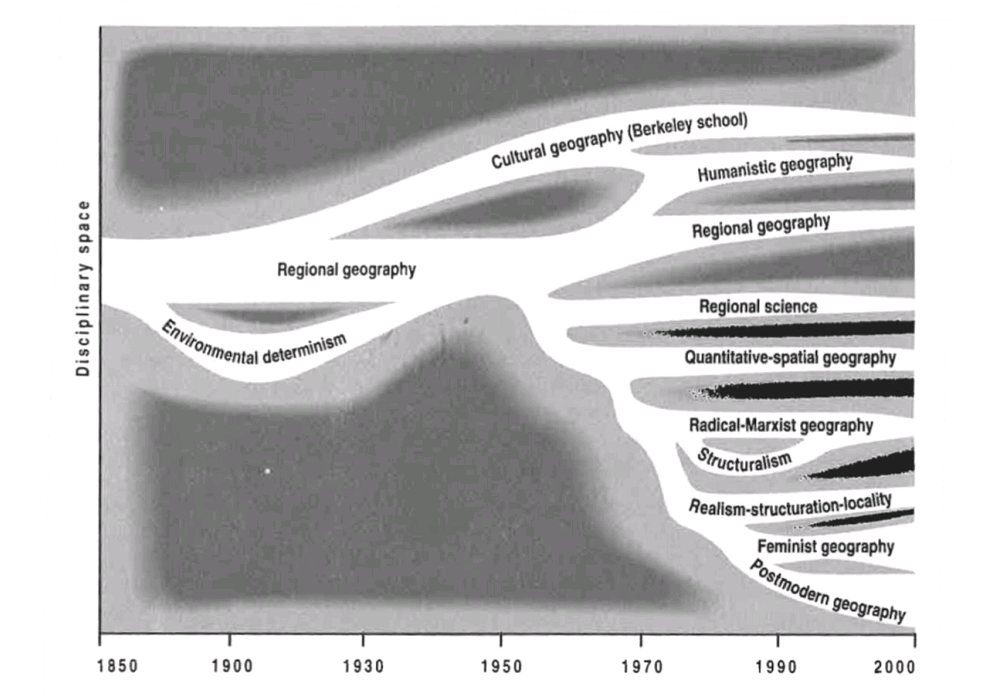
\includegraphics[width=23em]{geography_approaches.png}
\end{center}

\pagebreak\section{Theories of World-City Formation}

\textbf{Measuring centrality of cities/city-regions}:\alignedmarginpar{Deltametropolis, Flemish Diamond, RheinRuhr, Ile-de-France, Greater London}there are multiple ways to measure the power of cities or regions, like the weight of the area in the national context (regarding GRP, density...), the number of patents, the level of education, the proportion of employment per sector (higher in the service sector than industry or agriculture).

\textbf{World cities}:\alignedmarginpar{Friedmann}world cities are points of functional centrality, serving command and control functions in a global urban system, where processes cross national borders. The world economy is restructured, there is a new international division of labour (offshoring), TNCs and MNCs dominate the global supply chain that is highly integrated.
This creates uneven socio, economic and spatial developments because of a hierarchy connecting the core (absorbing the surplus) and the periphery.

\textbf{Global cities}:\alignedmarginpar{Sassen}path dependencies concentrate Advanced Producer Services in select cities. The path dependencies include the extensive services market providing access for firm/client relations, the labour market and associated culture, the APS complex and the cross-border connections offered by its network. 
APS have control capabilities and \textbf{polarise the labour market} (high and low-skilled labour required). This results in the \textbf{peripheralisation} of the core.

\textbf{Global city regions}:\alignedmarginpar{Scott\\Silicon Valley, Pearl River Delta}a complex assemble of cities, settlements, hinterlands that are interconnected by production networks, themselves oriented towards the global economy. An urban core is not always required for a region to be central in the post-Fordist industry (ie. service and knowledge industries). APS can still be an indicator for global city regions.

\textbf{GaWC heuristic}: used to map the world-city network. Assumption is that the presence of international APS firms can be used to indicate the presence of command-and-control functions of cities.

\textbf{Post-colonial critique}:\alignedmarginpar{Robinson} the western bias in urban knowledge production leaves places off the map of urban studies. Off the geographical map (global South), and off the conceptual map (limited economic processes, ignores inter-urban connections). World cities research ignores `ordinary' cities in the global economy.

\textbf{Social-constructivist critique}:\alignedmarginpar{Massey}the world-cities are politically constructed, and their consequences are un-debated and hide other realities\alignedmarginpar{London's financial centre vs. low-skilled labour}. World cities are not a given but a product of local and global forces, mediated by acts of representation (financial and political elites, or policies that promote the city).

\textbf{Political-economy critique}:\alignedmarginpar{Brenner}there is a rescaling of the state due to globalisation, which changes the political and economic scales to supra and sub-national levels. There are new governance structures, a shift from managerialism to entrepreneurialism\alignedmarginpar{inter-urban competition}, global accumulation regimes are centred on (global) cities, their importance reinforced by global city building agendas.

\textbf{Financialisation critique}:\alignedmarginpar{Bassens \& van Meeteren}the deregulation of financial markets has financialised firms who are mostly present in APS complexes. Unfortunately this leads to global financial crises, and tax evasions.

\pagebreak\section{Polarisation in World/Global Cities}

\textbf{Polarisation}:\alignedmarginpar{Friedmann and Wolf, citadel vs. ghetto}a class division that is reproduced through space, and is stronger in global cities. Polarisation is explained by an \textbf{economic restructuring}\alignedmarginpar{North-Atlantic}. Productivity has increased, but wages have not because profit is invested elsewhere (eg. financialisation)

\textbf{Economic restructuring}: post-Fordism restructured the economy. Production was relocated (globalisation, NIDL); deindustrialisation declined activity in the city; structural unemployment; shift towards fiscal austerity\alignedmarginpar{declining tax base}; market rationality and privatisation\alignedmarginpar{neoliberalism}; shift from state to market control over multinational capital; inter-urban competition.

\textbf{Harvey's entrepreneurial strategies}: \textbf{Production}: policy makers create/exploit certain advantages for the production of goods and services; forms clusters and edge cities. \textbf{Consumption}: improving the city's position in the spatial division of consumption; affects socio-spatial structure. \textbf{Redistribution}: competition for (supra)nationally redistributed surplus from the economy. \textbf{Command and control}: investing in high finance, government, and information economy; forms monopoly spaces in global/world cities.

\textbf{Polarisation thesis}:\alignedmarginpar{Friedmann \& Wolff; Sassen}the change in economic base led to a decline of well-paid manufacturing job (exodus) and a growth in service jobs (formal \& informal) with an influx of high-salaried workers (professional and managerial jobs) and low-skilled workers to support their lifestyle and routine service jobs. Creates an ``hourglass'' of ``upper circuit''/``underclass''.\alignedmarginpar{urban elite networks}

\textbf{Labour market globalisation}: global cities have high-paid and low-paid migrants, often divided ethnically.\alignedmarginpar{expat vs. immigrant} Growing supply of low-skilled migrant labour for typically 3D jobs (dirty, demanding/difficult, dangerous) drives wages down. There is growing informality and a \textbf{``peripheralisation at the core''}\alignedmarginpar{Sassen-Koob}, where exploitation not only takes place in the global South but also global North where the `peripheralised' live. \textbf{New forms of industrial exploitation} in \alignedmarginpar{sweatshops}global cities are made possible by the absence of regulation in the (global) periphery.

\textbf{Criticism of polarisation in global cities}: universalising and generalising tendencies, but does the logic apply elsewhere than NY-LON-TOK? Simplistic theory that reduces complexity of occupational and spatial structures, and professionalisation and mobility can also impact socio-spatial inequalities.

\textbf{Occupational structure}:\alignedmarginpar{Hamnett}professionalisation means high-income jobs are growing, and doesn't necessarily mean growth of low-paid jobs. There is an `upgrading' of the labour market, and better welfare states\alignedmarginpar{minimum wage} prevent extreme polarisation. Labour inequalities emerge because of market exclusion based on gender and ethnicity.

\textbf{Spatial structure}: statistics could exaggerate polarisation. Suburbanisation of the middle class could mean that middle-incomes are not disappearing but moving outside of the city. High-end housing demand drives super-gentrification\alignedmarginpar{Lees, 2003\\Brussels, Brooklyn}. Influence of pre-existing spatial forms and path dependencies. 

\textbf{Three-layer model}:\alignedmarginpar{Burgers and Musterd, 2000}for analysing inequality in cities: macro-level (global change, economic restructuring, increasing mobility of capital, people, commodities, information); micro-level (individual level, change in labour opportunities in a specific local context); medium-level (connects global and local, national institution differences, different urban trajectories)\alignedmarginpar{Charleroi/Detroit}

\textbf{Future}: income polarisation is expected to expand due to austerity, the flexibilisation of the labour market, migration labour, and political wealth.

\pagebreak\section{Urban Segregation: Patterns and Causes}

\textbf{Land-use model}:\alignedmarginpar{Burgess, 1925\\Chicago}an ideal type of 5 concentric circles shaped by the \textbf{bid rent theory}, whereby groups are able to pay different amount of rents (commerce/industry/residents). Density (and rent) decreases as one goes from the city centre towards suburbs. The model is of a growing city, in terms of population and built environment.

\textbf{Assumptions of land-use model}: assumes a cultural and social heterogeneity, a commercial and industrial economy, private ownership of property and economic competition for space, city expansion and population growth, equal mobility opportunities, CBD is the most valuable and the main centre for employment, attractiveness of districts is not based on terrain, no concentration of heavy industry, and not history survival of earlier land-use patterns in any district.

\textbf{Sector model}:\alignedmarginpar{Hoyt, 1939}a model for cities hit by socio-economic factors that slow population growth, in a society where cars play an increasingly important role. Sectors are organised around a core and grow outwards. Focus on social class rather than migrant groups.

\textbf{Multi-nuclei model}:\alignedmarginpar{Harris \& Ulman, 1945}a model where cities have a CBD, but also other strong areas with businesses and institutions.

\textbf{Alternative models}: the British city, the Chinese city, the African city (market zone, traditional CBD, colonial CBD), enclave urbanism (LA's skid row vs. gated suburbs), the post-socialist city.

\textbf{Provincialisation}: urban differentiation is characteristic of all cities. Urban form  is impacted by local features (topology, weather, socio-economic basis, migration patterns...) and local policies (transport systems, state interventions in housing, mobility restrictions, strategies to counter inequalities...). All land use models have birthmarks (time and place), and there is a need for provincialised (specific) theories about urban form and growth.

\textbf{Dimensions of (residential) segregation}:\alignedmarginpar{Massey \& Denton, 1988} the degree to which two or more groups live apart from each other in the urban environment. Dimensions are \textbf{evenness} (differential distribution of two social groups across space)\alignedmarginpar{index of dissimilarity}, \textbf{residential exposure} (degree of interaction opportunities between minority and majority groups in space), \textbf{concentration} (amount of physical space occupied by minority groups), \textbf{centralisation} (spatial distance from urban centre), \textbf{clustering} (extent to which minority-occupied areas adjoin one another in space). Scale matters!

\textbf{Causes of segregation}: different schools of thoughts on why different population groups occupy different parts of the city. \textbf{Quantitative spatial geography} uses ecological models of the city considered a natural area with homogeneous character, based on a pattern of expansion/competition/invasion/succession. \textbf{Radical-Marxist geography} uses flows of capital to understand where segregation fits. \textbf{Neo-Weberian geography} uses socio-economic constraints like financial, cognitive, political, social resources. \textbf{Behavioural geography} uses people's reasoning and preferences around living conditions and environments. \textbf{Post-modern geography} uses the meaning attached to home, and how it affects personal experiences.

\pagebreak\section{Neighbourhood Effects and Living with Diversity}

\textbf{Ideal of social mix}:\alignedmarginpar{Belgian cities, UK's HMR, USA, South Africa}popular amongst policy makers across the political spectrum. It supposes that where you live affects your life chances, such that residential segregation has a negative effect on the socio-economically disadvantaged, social mobility and cultural integration.

\textbf{Social mix feasibility}:\alignedmarginpar{Slater, Van Kempen \& Bolt} social mix policies don't resolve poverty, but displace people and move poverty elsewhere\alignedmarginpar{Brussels$\rightarrow$Charleroi}. Social mix that integrates different populations and helps rather than displaces is feasible, but hard to achieve in a market-dominant situation.

\textbf{Neighbourhood effects research}: bears birthmarks and needs to be \textbf{provincialised and contextualised}\alignedmarginpar{America vs. Europe}. Different researchers (ethno-cultural vs. socio-economic) have different approaches (qualitative vs. quantitative)

\textbf{Social network argument}: social capital is the connections and social networks that create reciprocity and trustworthiness between individuals.\alignedmarginpar{Strong \& weak ties} Living together creates bonding capital in socially homogeneous groups, and bridging capital between socially heterogeneous groups. BUT risks to disrupt existing bonding capital, and human extensibility\alignedmarginpar{Parallel lives}creates networks outside of neighbourhood

\textbf{Underclass argument}:\alignedmarginpar{Structuralists vs. Culturalists}poverty exists because of structural forces in a declining economic base, or because of a culture of poverty. Socialisation factors (peer groups, lack of role models) and institutional networks keep people in poverty. BUT are neighbourhoods really the cause?\alignedmarginpar{Uneven policing}Mobility and internet allow for socialisation outside the neighbourhood.

\textbf{Social cohesion argument}: living with natives creates opportunities for foreigners to integrate better. Using arguments of ethnic segregation and socio-economic mobility for social cohesion. BUT mobility means people can integrate outside neighbourhood, and local culture provides protective (arrival) spaces.

\textbf{Local services argument}: mixed neighbourhoods attract diverse shops and services. BUT differentiation creates differentiated demand that displaces specialised (ethnic) shops and services in arrival neighbourhoods, overshadows ethnic entrepreneurship which creates social mobility, and some may not find what they want.

\textbf{Political argument}:\alignedmarginpar{Environmental racism}mixed neighbourhoods will be higher on political agendas. BUT why don't politicians listen to low-income populations instead?

\textbf{Spatial mismatch argument}: disconnect between where people live (where poverty is concentrated) and low-skilled job opportunities. BUT is the problem social mix? Public transport gives people spatial mobility, and barriers like language prevent people from getting a job.

\textbf{Stigmatisation argument}: services and businesses hold stigmas and biases, and don't give as good a service or equal chances to poor residents.

\textbf{Conclusions}: social mix is not convincing. Instead of helping poor, ethnic minorities out of poverty, it displaces people and pushes gentrification. We need to ask: for whom is social mix? where and on what \textit{scale}? and what is the goal, and are there more effective alternatives? 

\pagebreak\section{Cultures of Urban Research}

\textbf{Cultural turn}: a shift in research practices in humanities and social sciences, to pay more attention to culture. Reasons are empirical (culture is increasingly important), theoretical (theories are required to better grasp cultural dimensions of social life), methodological (new and better methods are required to interpret (empirical) data, that isn't only number crunching).

\textbf{Postmodernism and the city}:\alignedmarginpar{Jameson,\\Bonaventura Hotel}postmodernism is the cultural expression of late capitalism, is a third stage of capitalism (post-industrial, late, multinational, consumer capitalism are the political economy of postmodernism). 
It isn't a style, but a cultural dominant, that entails a \textbf{commodification of culture}. Features are superficiality instead of depth; alienation of the subject because of fragmentation; historicism erasing history; culture is completely under influence of capitalism.

\textbf{LA School of Urbanism}: postmodern urbanism, characterised by urban fragmentation and sprawl, using LA as a prototype of future cities across the world, focused on restructuring (post-Fordism, flexible accumulation, Jameson's late capitalism). It has a diversity of claims and no core agreement.
Critiques are that it did not acknowledge ongoing research on diversity/restructuring/consumption/commodification/poverty; lacks ethnographies, relying on top-down interpretations; LA is not radically different; wrong to reduce Chicago School to Burgess' model.

\textbf{Keno capitalism}: an extreme interpretation of postmodernism, where keno capitalism is the manifestation of postmodern urbanism. A very fragmented urban structure, with no centre extending outwards, no central planning, `random' developments in the city. A parody that resonates today through the \textbf{cultures of heteropolis} and the \textbf{city as a theme park}.

\textbf{Urban landscapes and the symbolic economy}: another strand of research, using these guiding assumptions: the flexible accumulation and postmodernism are impossible to detach;\alignedmarginpar{Knox}the rise of postmodernism goes with the rise of a new middle-class and tastes; culture is key to urban redevelopment (artistic representation of urban space, gentrification);\alignedmarginpar{Zukin, Loft Living}important role of the state.

\textbf{Spatial turn}: increased interaction between the cultural and the spatial, ie. between urban geography, urban anthropology, and cultural studies. The core themes are \textbf{informality} and \textbf{everyday life}.

\textbf{Informality}:\alignedmarginpar{Hart\\Las Ramblas} of labour markets, precarious work, migration, legality, political governance and contestation. Informal/formal is different from illegitimate/legitimate. For example, household work is informal and legitimate, but drug dealing is informal and illegitimate. Related to unregistered economy, black market, non observed economy, undeclared work, shadow or hidden economy. 

\textbf{Everyday life}:\alignedmarginpar{Hall \& Jefferson\\Michel De Certeau} agency, building community, resistance, consumption, identity, media and representation. People are active, creative agents and not passive consumers. `Rural' concepts are applied. There is a focus on participant observation, extensive period of fieldwork to gain trust and inside knowledge of everyday practices. The `everyday' is a trans-disciplinary concept.

\pagebreak\section{Urban Cultures}

\textbf{Informality}:\alignedmarginpar{Keith Hart, Ghana}the distinction between formal and informal comes from the economy, and is the difference between the work that can and can't be taxed. Research focus is on: the opportunities and precarities of unregulated economic activities; the gendered dimensions of informal work; the transnational dimensions, including informal labour, migrant work being often transnational.  

\textbf{Everyday life}:\alignedmarginpar{H. Lefebvre, S. Hall, T. Jefferson}a trans-disciplinary concept connecting culture with philosophy, Marxism, ethnography, post-structuralism, sociology, aesthetics, etc. Since the 1980s, moving beyond community as a nostalgic concept. Key trends include conflicts over cohesion; network ties like care and support in dynamic urban contexts; shifting boundaries between communities because of conflict; elective belonging and subcultures which resist dominant social orders.\alignedmarginpar{Gay, gated communities}

\textbf{Arts, activism and urban engagement}: urban studies take a \textbf{sociological and/or political economic} approach to the arts and culture. There are different aesthetic strategies: spectacle, grassroots, social work, arousing dissensus... In practice, an artistic production can mix strategies, for example be both social work and spectacle.

\textbf{Public and site-specific art}:\alignedmarginpar{NYC art, Tilted Arc, Homeless vehicle}art can be used by local governments and developers as legitimate devices for uneven development. Art in a public space doesn't mean it addresses the public. It needs to engage with the public, in order to be public art. Public art needs to engage with people, engage with everyday practices and urban users in a constructive way.

\textbf{Artists and urban social movements}:\alignedmarginpar{Berlin/Hamburg squatting and demonstrations, BLM, F4F}artists often engage in social movements. Within urban studies, research has been centred around the creative class, neoliberal and entrepreneurial urbanism. Artists and cultural workers play a part in urban social movements, because they have a privileged role: they can access media networks, and use their (artistic)communication techniques to frame social movements.

\textbf{Popular culture and urban politics}:\alignedmarginpar{hip-hop}focuses on culture as/in everyday life, as questioning authority, as imagining political alternatives. It's about politics beyond government and politicians, towards a street politics and an informalisation of the state.

\textbf{Cultural infrastructures and informal urbanism}:\alignedmarginpar{Larkin, Signal and Noise}on the symbolic and representational logic of infrastructure. What does infrastructure mean, how is it represented, how/what does it envision? Governments have an incentive to control infrastructures, and infrastructures have unexpected outcomes. Informal social and everyday practices happen around these infrastructures.

\textbf{Analytical shift in cultural infrastructures and informal urbanism}: from informal economy and everyday life tactics, to informal urbanism. A wide variety of topics, like DIY urbanism, co-working space, co-housing, squatting, self-built housing... Informal urbanism transcends north/south divides, and is global urbanism. 

\textbf{Sensory urbanism, visual cultures and sounds}:\alignedmarginpar{LaBelle}media technologies and aesthetics shape urban places, such that places are experienced with all senses. For example through starchitecture, city branding, cultural tourism, social media, and all the sounds of a city like crosswalks signals.

\pagebreak\section{Transport and Cities: a Historical Hegemony}

\textbf{Transport and urban form}:\alignedmarginpar{Does the city shape transport, or does transport shape the city?}urban development is intricately linked with transport technology. Transport evolved from the pre-industrial city (walking), industrial city (tramway), fordist city (car)\alignedmarginpar{Massification}to post-fordist city (air, ICT).
New transport changed the urban form: an increased operating speed meant increased coverable distance; the city expanded (suburbs) and connected (villages); there was specialisation of economic functions (new working class, new social groups); people could commute (separate home and work); major infrastructure projects took place and nation-wide programs developed (with resistance), and urban planning strategies promoted cars over public transport, which were focused on suburbs.\alignedmarginpar{Storkøbenhavn}

\textbf{Colonisation of space}: with the creation of the metric system, the state was able to create the socio-economic developments like electricity, water, rail, etc. infrastructures. This colonisation of space not only exists on a national scale, but a global scale. Around the `colonisation' of measuring systems, sciences developed: transport engineering and transport economies, and neoclassical economics (supply and demand).

\textbf{Neoclassical transport}: has two general principles, the rationality of transport, and transport as a motor of economic growth.

\textbf{Rationality of transport}: transport is purely technical, expert-led, reduced to universal measures, cannot be debated. It assumes that the user is a rational being (homo economicus) who chooses the most efficient way to get to a destination, and is making purely utilitarian travel choices.

\textbf{Transport as a motor of economic growth}: assumes that any improvement to transport infrastructure leads to higher speeds and lower travel times, thus to lower transaction costs, and that transport development creates urban economic development, and vice-versa. It monetises travel time, labelling it as unproductive, but transportation need mustn't be monetarily unproductive.\alignedmarginpar{Cycling for leisure}The key problem for urban transport is to overcome congestion: any obstruction to the fluid flow of cars needs be solve because it is otherwise \textbf{irrational} and \textbf{hampers economic growth}.

\textbf{Critique of neoclassical transport}: it is devoid of social, theoretical and political discussions. People are not purely objective beings (homo-economicus), but are nuanced (age, gender, abilities, class, ethnicity). Concepts like anti-capitalist, Marxist, feminist theories are absent from engineering discourses, and transport is based on increasingly complicated mathematical models on human behaviour.

\textbf{Transport supply and demand}: technical, quantitative measures of transportation. Supply is the capacity of transportation infrastructure (space and time), and the demand is expressed in people, volume, or weight per unit of space and time.

\textbf{The city in neoclassical transport}: reduced to a field of application, rather than the outcome of socio-economic, political and spatial dynamics. Inefficient (pre-industrial) elements should be removed in order to apply new models, and the city is a playground for technical and rational solutions. Problems like congestion must be solved with more infrastructure, or risk being a detriment to the economy.

\textbf{Sustainable urban transport}: transport is locally and globally the leading source of emissions. There is a growing population and an increase in urban mobility, but a growing demand for cars. Thus, climate problems are increasingly transport problems, and transport problems are increasingly urban problems.

\pagebreak\section{Critical Perspective on Urban Transport}

\textbf{Sustainable mobility paradigm}:\alignedmarginpar{Banister}need to break with mono-functionalism and engage in mixed planning practices, where different functions exist near each other in order to reduce travel times. Need to facilitate the modal shift away from unsustainable transport (car) by supporting public transport, collective mobility and soft transport. This can be done by moving away from top-down policy and planning, and paying attention to individual behaviours and lifestyles,\alignedmarginpar{Citizen participation}including transport accessibility and social inclusion.

\textbf{The city in the sustainable transport paradigm}:\alignedmarginpar{Jacobs, Bannister}sustainable transport is an integral component of a ``good city''. It is economically performing (modal shift from cars does not destroy the economy), it creates social cohesion and diversity, is environmentally friendly and participative.

\textbf{Tackling automobility}:\alignedmarginpar{Congestion charge, reduced infra, no-car zones, BRT}can be achieved by improving vehicle technology, restricting car accessibility, increasing public transport quality/accessibility, and promoting multi-modality so people have options besides the car, and choose based on behaviours and lifestyle.

\textbf{Reducing travel needs}:\alignedmarginpar{Reigner}can be achieved by promoting proximity and density, ICT,\alignedmarginpar{tele-work, tele-shopping}, trip substitution and trip switching, shared transport. These are `radical' interventions that renew the city, making it more sustainable and attractive and giving it back to the people.

\textbf{Key problem}: neoclassical and sustainable perspectives dominate urban transport, and sustainability has been appropriated by car and oil industries. This can only take `sustainability' so far, and is an unproductive debate. We need to deconstruct sustainable urban transport and explore critical perspectives.

\textbf{Deconstructing sustainable transport}:\alignedmarginpar{Clean cars, underground motorways}there is \textbf{technological determinism}, thinking that technological innovation will resolve the problem, and no attention given to socio-political innovations like incentives for public transport. A \textbf{moralising perspective}\alignedmarginpar{Reigner} focusing on pedagogics over politics, convincing people to change their mobility habits, but is revanchist moral geography which ignores the structural causes behind transport behaviours. An \textbf{uneven geography}\alignedmarginpar{Car-free cities, congestion charges\\Oslo, Madrid, Brussels}where the city is saved from the car, but car infrastructure proliferates in peripheries and underground. \textbf{More participation but less power}, sustainable transport should embrace a diversity of stakeholders but the dominant actors decide over the dominated. There is an \textbf{emphasis on transport rather than on the urban}, emphasising successful outcomes rather than broader, structural urban implications.

\textbf{Exploring critical approaches}: explores global neoliberalisation trends in transport; the link between gender, race and class; transport-related socio-spatial inequalities and exclusions; transport as places of contestation and urban movements; challenge neoclassical-sustainable hegemony; inter-urban competition; relation with labour markets.

\textbf{New mobilities paradigm}:\alignedmarginpar{Sheller and Ully}transport shifts from  infrastructure towards a social consideration, and looks at mobility as the base to everyday life. Critique is that it ignores the macro-politics of mobility (structural issues) and power dynamics.

\textbf{Urban political economy of transport}:\alignedmarginpar{Harvey, Smith, Soja\\anti-neoliberal}considers the city as a social and political construct, not governed by rational or natural processes. Aims to understand and challenge the social, political and economic structures behind unsustainable contemporary transport policies and practices. Transport is a structural phenomenon and a form of capital, unevenly distributed across space, and discriminatory. People mobility behaviour is shaped by the politico-economic system, and not their lifestyle.

\pagebreak\section{Glossary}

\textbf{Post-fordism}: the idea that modern industrial production has moved away from mass production in huge factories, towards specialised markets based on small flexible manufacturing units

\textbf{}





\end{document}
